\section{Základní podstata zvětrávání}
Zvětrávání je změna fyzikálních a chemických vlastností hornin po jejich obnažení na zemském povrchu. Produktem \emph{zvětrávacích procesů} jsou \emph{zvětraliny}. Ke změnám vlastností hornin dochází z důvodu odlišných fyzikálně-chemických podmínek při vzniku horniny a na zemském povrchu. Čím odlišnější podmínky panovaly při vzniku dané horniny, tím náchylnější je ke zvětrávání. Maximální možný dosah zvětrávacích procesů se udává okolo \SI{1}{\kilo\metre} do hloubky. Zvětrávání hornin je přípravou pro další procesy.

\section{Fyzikální (mechanické) zvětrávání}
Při fyzikálním zvětrávání dochází k rozrušování horniny a rozpadu na menší částice. Mění se tedy fyzikální vlastnosti hornin a ne chemické složení. U některých typů fyzikálního zvětrávání dochází až k rozpadu na jednotlivá minerální zrna. Příčinou jsou vždy změny objemu v horninovém masivu

\subsection{Změny teplot}
Horniny a minerály jsou špatným vodičem tepla. Při oslunění skalního povrchu se tak během dne prohřeje jen pár svrchních centimetrů. Zároveň s růstem teploty horniny roste i její objem. Dramatické rozdíly mezi teplotou na povrchu a uvnitř tak způsobují pnutí v hornině, což vede k odlupování tenkých slupek hornin (tzv. \emph{deskvamace}). Rozdílná teplotní roztažnost minerálů může způsobit vypadávání jednotlivých minerálních zrna tzv. \emph{odzrňování}. Prudké zahřátí povrchu vlivem např. lesních požárů způsobuje \emph{termické pukání} hornin. Silné ochlazení může naopak vyvolat \emph{mrazové pukání}.

% TODO: \usepackage{graphicx} required
\begin{figure}
	\centering
	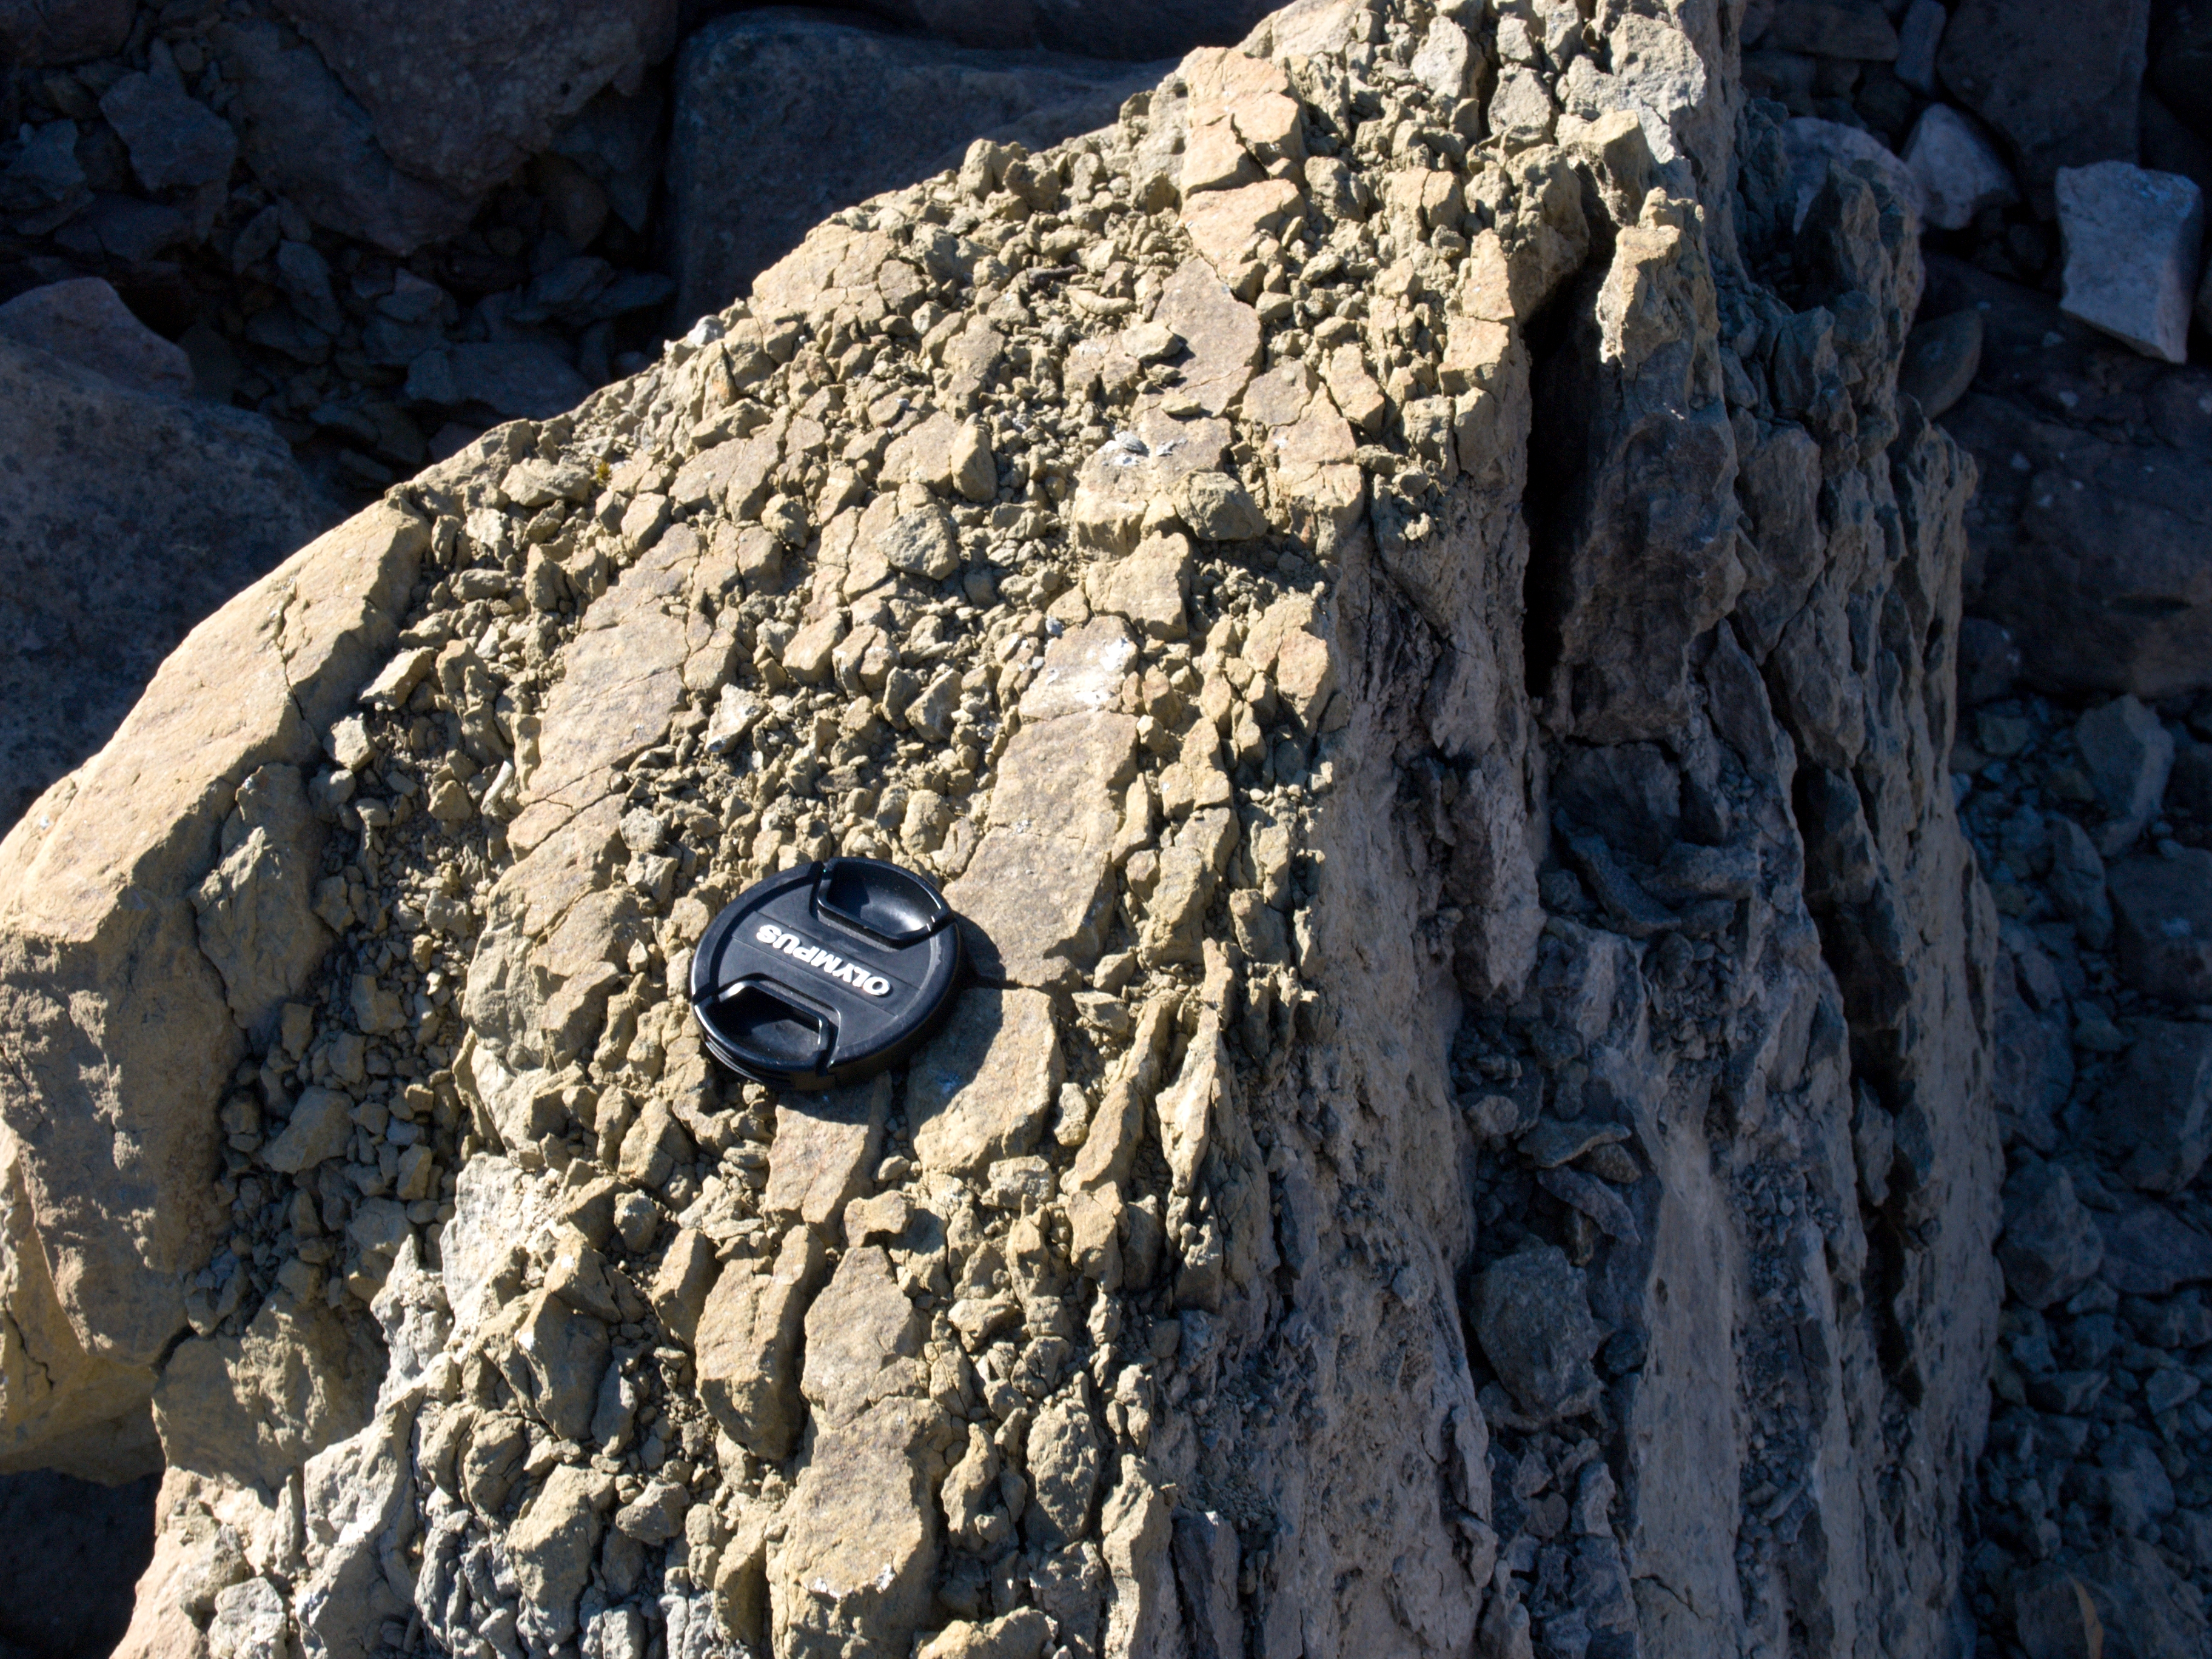
\includegraphics[width=1\linewidth]{obrazky/zvetravani/mrazove}
	\caption{Ukázka mrazového tříštění, Svalbard.}
	\label{fig:mrazove}
\end{figure}

\subsection{Fyzikální zvětrávání vlivem růstu krystalů}
Růst krystalů způsobuje objemové změny v horninách a jejich následné tříštění. Voda když zmrzne zvětší svůj objem o necelých $\SI{9,08}{\percent}$, což vede k postupnému rozšiřování puklin a tříštění hornin (\emph{gelivaci}). Prodkutem \emph{makrogelivace} jsou například kamenná moře. \emph{Mikrogelivace} způsobuje oddělování jednotlivých zrn horniny (produkt je kryopelit).


K tříštění hornin dochází i růstem krystalů soli z roztoků. \emph{Solné tříštění} se hlavně uplatňuje u pórovitých hornin (např. pískovců) v aridních či příbřežních oblastech.

Objemové změny krystalů mohou nastávat i z důvodu některých chemických změna (např. hydratace, dehydratace či oxidace).

\subsection{Fyzikální zvětrávání vlivem odlehčení (exfoliace)}
\emph{Exfoliace} je proces při kterém se z výchozů skalního podloží odlupují horninové slupky rovnoběžné s povrchem. Exfoliační pukliny vznikají z důvodu odlehčení hornin. Odstraněním nadloží se totiž v horninách uvolňuje napětí, které bylo indukované tíhou nadložních hornin. Nejčastěji jsou tyto pukliny při povrchu, avšak byly nalezeny i několik desítek metrů pod povrchem.
Mocnost exfoliačních slupek se zpravidla pohybuje od 0,5 do \SI{10}{\metre}, v takovém případě hovoříme o \emph{makroexfoliaci}. Odlupování tenčích slupek (v řádu \si{mm} až \si{cm}) označujeme jako \emph{mikroexfoliaci}.

Exfoliací vznikají exfoliační klenby. Nízké se nazývají \emph{ruwary}, vysoké \emph{bornhardty}.

% TODO: \usepackage{graphicx} required
\begin{figure}[h]
	\centering
	\includegraphics[width=1\linewidth]{obrazky/zvetravani/exfoliace}
	\caption{Ukázka exfoliace žuly. Half Dome v Yosemitském národním parku. (Autor: Ronnie Macdonald, CC BY 2.0 )}
	\label{fig:exfoliace}
\end{figure}


\section{Chemické zvětrávání}
\emph{Chemické zvětrávání} (také rozklad nebo dekompozice) je změna chemických vlastností hornin a jejich minerálů. Dochází k nahrazení stávajících minerálů jinými. Změna chemických vlastností je provázena i zvětšením objemu a zmenšením hustoty minerálů. Základní podmínkou pro chemické zvětrávání je \emph{přítomnost vody} a dostatečná \emph{teplota}.

Minerály, který vznikaly při podmínkách značně odlišných od těch co panují na zemském povrchu, zvětrávají rychleji, než ty které vznikaly za podmínek podobných. Tmavé (mafické) minerály zvětrávají na zemském povrchu rychleji než světlé (felsické) minerály. Tedfy olivín a pyroxen zvětrává rychleji než muskovit či dokonce křemen. Tzv. \emph{Goldichovo pravidlo zvětrávání} je v podstatě obráceným \emph{Bowenovým krystalizačním schématem}, které znázorňuje pořadí minerálů krystalizujících z postupně chladnoucího magmatu. Ty minerály, které krystalizují př nejvyšších teplotách naopak nejrychleji podléhají zvětrávání. Samozřejmě v přírodních podmínkách to je poněkud komplikovanější. 

Mobilita kationtů v minerálech ovlivňuje jak rychle se uvolní daný prvek z horniny, jak dlouho zůstává rozpuštěný ve vodě. Pořadí od nejmobilnějších k těm nejméně mobilným: \ce{Ca^2+, Na+, Mg^2+} $>$ \ce{K+} $>$ \ce{Fe^2+} $>$ \ce{Si^4+} $>$ \ce{Fe^3+} $>$ \ce{Al^3+}. Nejmobilnější kationy (\ce{Ca^2+, Na+, Mg^2+}) jsou první, které jsou z hornin vyplavovány. Naopak málo mobilní kationy ajko je \ce{Si^4+, Fe^3+, Al^3+} zůstávají ve zvětralině, kde dochází postupně ke zvyšování jejich koncentrace. 

\subsection{Typy chemického zvětrávání}
Nejjednodušším typem chemického zvětrávání je \emph{rozpouštění}. Rozpustnost minerálů je závislá na teplotě, pH a ale také i na rychlosti proudění vody v horninových pórech. Například dešťová voda je díky rozpuštěnému \ce{CO2} lehce kyselá (pH = 5,7). Významné je rozpouštění vápenců, které vede ke vzniku krasových oblastí a výzdob. 
%\subsubsection{Rozpouštění}
%Jedná se o nejjednodušší typ chemického zvětrávání. Rozpustnost minerálů je závislá na teplotě a pH vody.
%
%\subsubsection{Hydrolýza}

Dalším typem chemického zvětrávání je \emph{hydrolýza}. Ionty vody (\ce{H+} a \ce{OH-})  Molekula vody se dělí na proton (\ce{H+}) a hydroxidový aniont (\ce{OH-}). Vodíkový kation nahrazuje v krystalické mřížce kationy kovů (\ce{K+, Na+, Ca^2+, Mg^2+}) a ty se sluřují s hydroxidovým aniontem a stávají se součástí roztoku. Hydrolýza je hlavním procesem zvětrávání u silikátových hornin.

\emph{Oxidace} je typem reakce, při které prvek nebo sloučenina ztrácí jeden elektron (zvyšuje se tak jeho oxidační číslo). Například železnaté sloučeniny se oxidují na železité (\ce{Fe^2+} na \ce{Fe^3+}). Oxidačním činitelem nemusí být jen kyslík, ale například trojmocné železo, čtyřmocný mangan aj., zkrátka ty ionty, které jsou schopny přijmout elektron od oxidované sloučeniny. Oxidace je dominantní u minerálů, které obsahují \ce{Fe} (pyrit, siderit atd.), ale také \ce{Al}, \ce{Mg}, \ce{Mn}, \ce{Cr}. Opakem oxidace je \emph{redukce}. Redukovaná sloučenina přibírá elektron. Redukčním činitelem jsou ty ionty, které mohou elektrony předávat (např. dvojmocné železo, dvojmocný mangan). Projevy oxidace a redukce lze ve zvětralině či půdě poznat podle barvy. Hnědé či červené zbarvení poukazuje na oxidační prostředí, jelikož je typickým znakem oxidů trojmocného železa, kdežto šedá až šedozelená barva je typická pro redukční prostředí.


\emph{Hydratace} označuje proces obohacování minerálu vodou. Ta se dostává do krystalické mřížky. Sloučenina, která přijímá vodu, zvětšuje svůj objem a tím může mechanicky působit na své okolí. Opakem tohoto procesu je \emph{dehydratace}.

\emph{Karbonatizace} je reakce za účasti hydrogenuhličitanového anionu (\ce{HCO3^-}). Ten se nachází ve vodě v důsledku rozpoučtění \ce{CO2} ve vodě a následné disociace kyseliny uhličité (\ce{H2CO3}): 
\ce{H2O + CO2 <-> H2CO3 <-> H^+ + HCO3^-}
Karbonatizace je důležitá pro zvětrávání vápenců (reakce krasovění).

\emph{Lateritizace} je proces, který je vázán na monzunové vnější tropy, kde je vyhraněné období sucha a vlhka. Během vlhkého období dochází k intenzivnímu rozpouštění minerálů a následné migraci \ce{Fe} a \ce{Al} v roztoku a jejich relativnímu hromadění v různých hloubkách pod povrchem. Intenzivní výpar během sucha naopak způsovuje, že \ce{Fe} a \ce{Al} se hromadí při povrchu v podobě sesquioxidů, které vytváří pevné kůry -- laterity.

\begin{figure}[h]
	\centering
	\includegraphics[width=1\linewidth]{obrazky/zvetravani/laterit}
	\caption{Zvětrávání bazaltového tufu (bílá barva) do saprolitu (žluto-bílá) a lateritu (tmavě hnědá), Vangaindrano, Madagascar (Zdroj: Werner Schellmann, CC BY-SA 2.5, via Wikimedia Commons)}
	\label{fig:laterit}
\end{figure}


\emph{Kaolinizace} je typický proces ekvatoriální humnidní zóny. Jedná se o dlouhodobé zvětrávání ve slabě kyselém prostředí. Důležité je velké množství srážek a možnost odtoku vody. Dochází k silném rozkladu původní strktury minerálů (živec, slída...). V místě zůstávají stabilnější prvky (\ce{Si} a \ce{Al}). Produktem jsou kaolinické zvětraliny (kaolinit).
%
%\subsubsection{Karbonatizace}
%Reakce minerálů s \ce{CO2} rozpuštěným ve vodě
%Vzniká aniont \ce{HCO3-} (nejčastější aniont v povrchových vodách)
%Dominantní zvětrávací proces u karbonátů (zvratná reakce)
%
%\subsubsection{Lateritizace}
%Proces vázaný na monzunové vnější tropy s vyhraněným obdobím sucha a vlhka
%Ve vlhkém období dochází k intenzivnímu rozpouštění a relativnímu hromadění 
%V období sucha dochází k výparu a \ce{Fe} a \ce{Al} se hromadí při povrchu jako sesquioxidy – tvoří pevné kůry při povrchu – laterity (bauxity)
%
%\subsubsection{Kaolinizace}
%Proces typický pro ekvatoriální humidní zónu
%Podmínky: 
%Dlouhodobé zvětrávání ve slabě kyselých podmínkách (nejmenší rozpustnost kaolinitu)
%Intenzivní srážky a možnost odtoku vody
%Silný rozklad původní struktury minerálů (živec, slída - alumosilikáty) - zůstávají stabilnější prvky - 
%Produkty – kaolinické zvětraliny (kaolinit)




%\subsubsection{Oxidace}
%Zvětrávání minerálů, které obsahují \ce{Fe} (pyrit, siderit atd.), ale také \ce{Al}, \ce{Mg}, \ce{Mn}, \ce{Cr}. (u těchto hornin je dominantní)
%Oxidovaná sloučenina ztrácí jeden elektron, 
%Reakcí sloučeniny s ve vodě rozpuštěným O2 dochází ke zvětšení objemu sloučeniny
%Vznikají oxidy a hydroxidy železa (většinou nerozpustné) – červená nebo žlutá barva (goethit, limonit, hematit)
%Exponované jsou horniny, které obsahují minerály s příměsí železa (pyroxeny, amfibolit, biotit) – červené povlaky na obnažených stěnách
%Příklad: 
%
%\subsubsection{Redukce}
%Opak oxidace – snížení oxidačního čísla 
%(\ce{Fe^3+} na  \ce{Fe^2+})
%Dochází k ní v prostředí s nedostatkem volného kyslíku
%Průběh v zamokřených zónách (např. močály atd)
%Výsledkem jsou látky chudé na kyslík – pyrit, markazit a jiné sloučeniny šedého, šedozeleného a modrého zbarvení

%\subsubsection{Hydratace a dehydratace}
%Včlenění vody do struktury sloučeniny
%Sloučenina, která přijímá vodu, zvětší svůj objem a tím může mechanicky působit na své okolí
%
%Příklad: Anhydrit x Sádrovec
%
%\ce{CaSO4 <--> CaSO4.2H20}
%

%\begin{myboxgreenwide}{Příklady rovnic chemického zvětrávání}[h]
%\textbf{Rozpouštění}: \\
%\ce{SiO2 + 2H2O -> Si(OH)4}\\
%
%\textbf{Hydrolýza:} \\
%\ce{$\underset{\text{ortoklas}}{\ce{2KAlSi3O8}} + 
%	\underset{\text{kys. uhličitá}}{\ce{2H2CO3}} + 
%	\underset{\text{voda}}{\ce{9H20}}$ -> \\
%	->
%	$\underset{\text{kaolinit}}{\ce{Al2Si2O3(OH)4}} + 
%	\underset{\text{kys. křemičitá}}{\ce{4H4SiO4}}  + 
%	\underset{\text{kationt draslíku}}{\ce{2K+}}  +
%	\underset{\substack{\text{hydrogenuhličitanový aniont}}}{\ce{2HCO-3}} $}
%
%\textbf{Oxidace:}\\
%\ce{4Fe^2+ + 3O2	->	2Fe2O3}
%
%\textbf{Hydratace a dehydratace} \\ Anhydrit x Sádrovec
%\ce{CaSO4 + 2H2O <--> CaSO4.2H20}
%
%\textbf{Karbonatizace} \\ Rozpouštění kalcitu
%\ce{CaCO3 + H2CO3 <-> Ca2+ + 2(HCO3^-)}\\
%\end{myboxgreenwide}


\section{Biologické zvětrávání}
Zvětrávání v důsledku činnosti organismů může mít charakter fyzikálního, ale i chemické zvětrávání. Pod fyzikálním biologickým zvětráváním si snadno můžeme představit růst kořenů rostlin, a jejich rozrušování hornin (rozšiřování puklin mezivrstevních spár apod.). Chemické zvětrávání je pak způsobené např.  Chemické zvětrávání organismy spíše urychlují (např. zvýšené množství \ce{CO2} v důsledku dýchání). 

\section{Zvětralinová pokrývka}
Produktem zvětrávání je zvětralinová pokrývka. Její podoba je odvislá na typu zvětrávání. Fyzikální zvětrávání produkuje hrubší, ostrohranný materiál a naopak produkty chemického zvětrávání jsou daleko jemnější a mají hlinitojílovitý charakter. Mocnost zvětralinové pokrývky souvisí s charakterem podnebí, délce zvětrávání a samozřejmě s odolností horniny. Na svazích je mocnost zvětraliny menší než na rovinách. Zvětralinu, která je na místě svého vzniku (\textit{in situ}) označujeme jako \emph{saprolit}, naopak zvětralina, která je gravitašně přesouvána z vyšších částí svahu se nazývá \emph{regolit}.

%\subsection{Zvětrávání a klima}
%\emph{Vlhké tropy a subtropy} jsou příznivé pro intenzivní chemické zvětrávání. Mocnost zvětraliny může dosahovat i stovek metrů. Díky vysoké organické aktivitě je voda v půdě značně kyselá (obohacena o \ce{CO2} a organické kysleiny), což způsobouje rozpouštění a vymývání \ce{Na+, Ca^2+, Cl+, Mg^2+} a dalších rozpustných složek. Naopak se tam hromadí nepohyblivé prvky \ce{Fe^3+, Al^3+}.
%
%\emph{Semiaridní a aridní oblasti}
%
%\emph{Mírné pásmo}
%
%\emph{Subpolární pásmo a vysokohorské prostředí}
%
%%\subsection{Produkty chemického zvětrávání}
%%Zvětralinový plášť, zvětrávací kůry
%%
%%\subsubsection{Typy zvětralinových kůr}
%%Zpevněné polohy ve zvětralinách, které se vyskytují na zemském povrchu nebo těsně pod ním
%%Vznikají aktivním nebo pasivním hromaděním některých prvků a sloučenin 
%%Pasivní akumulace (u málo mobilních prvků)
%%Ferricrete (hromadění Fe)
%%Alcrete (hromadění Al)
%%Aktivní akumulace (v případě mobilních prvků)
%%Silcrete (nad95 \% \ce{SiO2})
%%Calcrete (nad 80 \% \ce{CaCO3})
%%Gypscrete (nad 95 \% \ce{CaSO4.2H2O})
